\section{Fungsi basis Lagrange}

Untuk suatu interval $[0,L_{\alpha}]$ yang diberikan, dengan $L_{\alpha} > 0$, titik grid
$x_{\alpha}$ sesuai untuk fungsi basis
Lagrange periodik dapat dinyatakan dengan persamaan berikut.
\begin{equation}
x_{\alpha} = \frac{L_{\alpha}}{2}\frac{2\alpha-1}{N_{a}}
\end{equation}
Fungsi basis Lagrange periodik yang akan digunakan
memiliki bentuk sebagai berikut.
\begin{equation}
\phi_{\alpha}(x) = \frac{1}{\sqrt{N_{\alpha}L_{\alpha}}}
\sum_{n_{\alpha}=1}^{N_{\alpha}} \cos\left[
\frac{\pi}{L_{\alpha}}(2n_{\alpha} - N_{\alpha} - 1)(x-x_{\alpha})
\right]
\end{equation}

Test
\begin{figure}
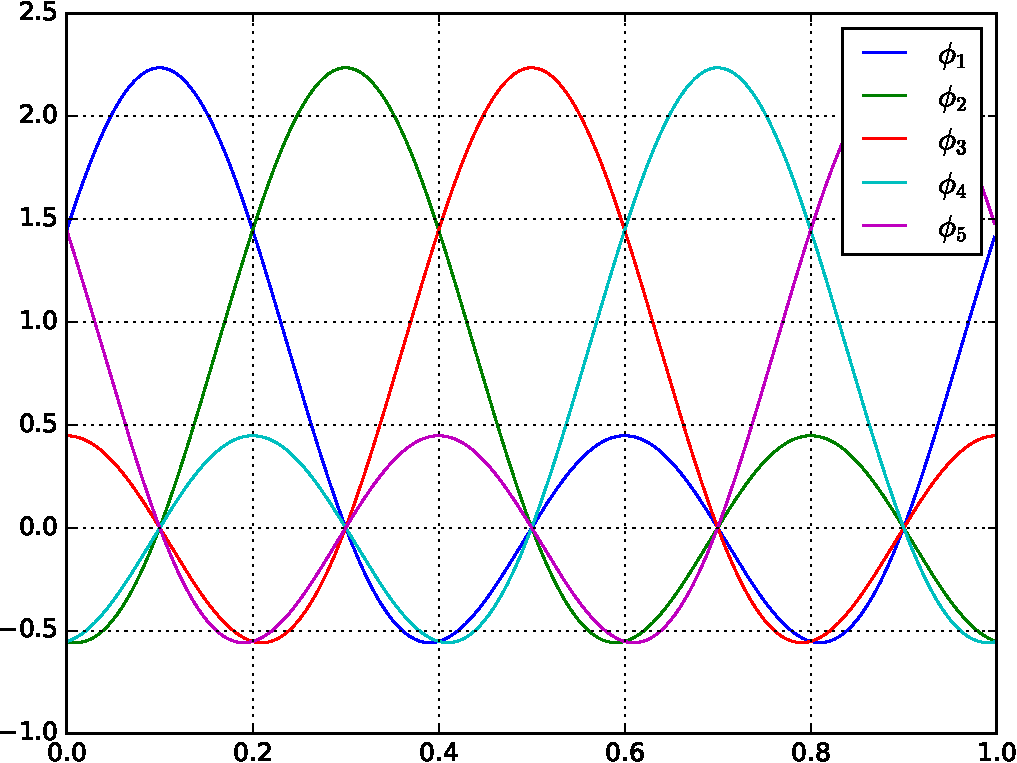
\includegraphics[scale=0.5]{images/plotN_5.pdf}
\end{figure}

Sembarang fungsi periodic $f(x) = f(x+L_{\alpha})$ dapat diekspansi dalam fungsi basis
Lagrange
\begin{equation}
f(x) = \sum_{\alpha}^{N_{\alpha}} c_{\alpha} \phi_{\alpha}(x)
\end{equation}
dengan $c_{\alpha}$ adalah koefisien ekspansi.
Nilai fungsi $f(x)$ pada titik grid $x_{\alpha}$ dapat diperoleh langsung
dari koefisien ekspansi melalui hubungan
$c_{\alpha} = \sqrt{L_{\alpha}/N_{\alpha}}f(x_{\alpha})$.

Ekspansi persamaan Kohn-Sham dengan fungsi basis Lagrange:
\begin{equation}
\psi_{i}(\mathbf{r}) = \sum_{\alpha\beta\gamma}
C^{i}_{\alpha\beta\gamma} \Phi_{\alpha\beta\gamma}(\mathbf{r})
\end{equation}
dengan fungsi basis \cite{Baye2015}
\begin{equation}
\Phi_{\alpha\beta\gamma}(\mathbf{r}) =
\phi_{\alpha}(x)\phi_{\beta}(y)\phi_{\gamma}(z)
\end{equation}
